% NOTES:
%   - Existing approaches answer the "what are the alternatives?" question from the problem statement
%   - Usage patterns motivate what SolidSessionBench simulates (sessions, interests, refinement)

\begin{frame}{Existing Evaluation Approaches}
  \begin{columns}[T]
    \begin{column}{0.6\textwidth}
      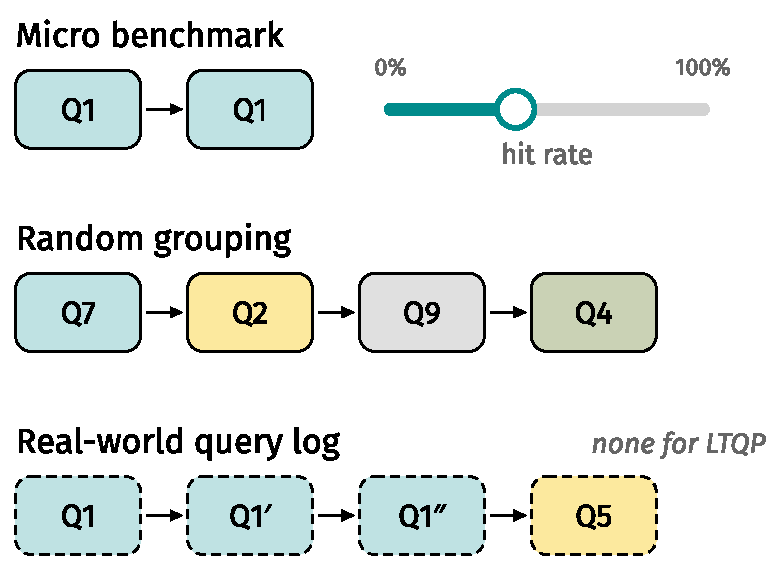
\includegraphics[width=\linewidth]{images/evaluation-approaches.pdf}
    \end{column}

    \begin{column}{0.4\textwidth}
      \begin{itemize}
        \item Micro benchmarks isolate single variables \parencite{hartig2011caching,nicholson2024hpcache}
        \item End-to-end benchmarks group unrelated queries \parencite{bizer2011berlin,martin2010improving}
        \item Real-world query logs are the gold standard \parencite{saleem2015lsq}, but none exist for LTQP
      \end{itemize}
    \end{column}
  \end{columns}
\end{frame}

\begin{frame}{Towards a Shared Simulated Benchmark}
  \begin{itemize}\setlength\itemsep{1em}
    \item Next best option: a unified simulated benchmark
    \item Common basis for comparison and improved reproducibility
    \item Grounded in usage patterns observed in the literature:
      \begin{itemize}
        \item User interest-based query behavior
        \item Logical query sessions
        \item Query refinement
      \end{itemize}
  \end{itemize}
\end{frame}

\begin{frame}{Usage Patterns: User Interest-Based Query Behavior}
  \begin{columns}[T]
    \begin{column}{0.6\textwidth}
      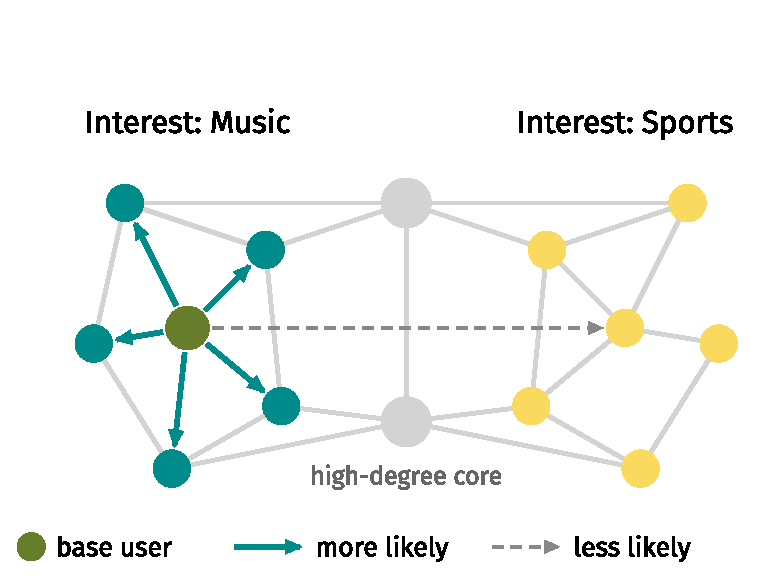
\includegraphics[width=\linewidth]{images/user-interests.pdf}
    \end{column}

    \begin{column}{0.4\textwidth}
      \begin{itemize}
        \item Users form communities based on shared interests \parencite{mislove2007measurement}
        \item Shared interests drive more interactions between users \parencite{mitzlaff2013user}
        \item[$\Rightarrow$] Simulate user-relatedness when choosing what to query
      \end{itemize}
    \end{column}
  \end{columns}
\end{frame}

\begin{frame}{Usage Patterns: Logical Query Sessions}
  \begin{columns}[T]
    \begin{column}{0.6\textwidth}
      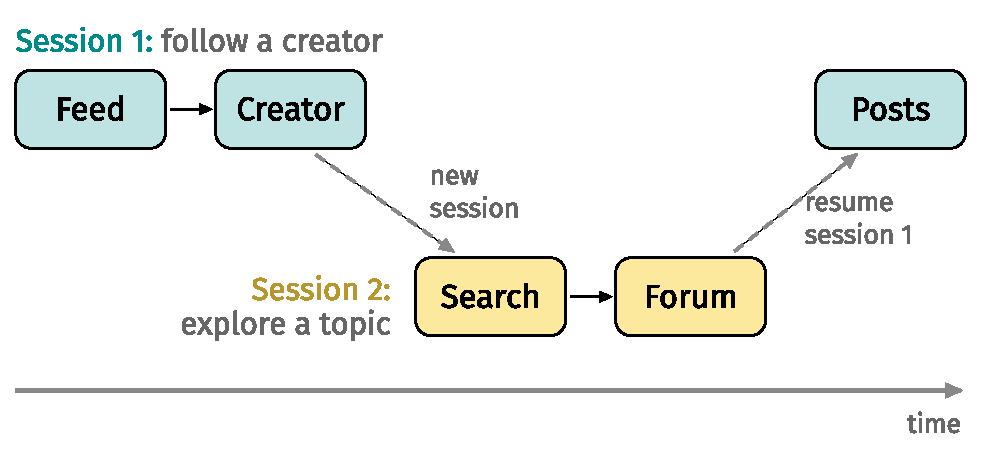
\includegraphics[width=\linewidth]{images/logical-sessions.pdf}
    \end{column}

    \begin{column}{0.4\textwidth}
      \begin{itemize}
        \item Browsing is grouped into goal-oriented logical sessions \parencite{meiss_whats_2009}
        \item New sessions begin in approximately 15\% of clicks
        \item Next query builds on previous results
        \item[$\Rightarrow$] Simulate dependent queries and session switching
      \end{itemize}
    \end{column}
  \end{columns}
\end{frame}

\begin{frame}{Usage Patterns: Query Refinement}
  \begin{columns}[T]
    \begin{column}{0.55\textwidth}
      \begin{block}{SPARQL query logs \parencite{bonifati2020analytical}}
        \begin{itemize}
          \item Related queries are issued in streaks
          \item Iteratively refined towards a shared goal
          \item Mostly adding or removing \texttt{FILTER}, \texttt{UNION}, and \texttt{OPTIONAL}
        \end{itemize}
      \end{block}
    \end{column}
    \begin{column}{0.4\textwidth}
      \begin{block}{Exploratory querying \parencite{arenas2025exploring}}
        \begin{itemize}
          \item Result refinement
          \item Result generalization
          \item Result extension
          \item Bug fixing
          \item Query refinement
          \item Shifting query intent
        \end{itemize}
      \end{block}
    \end{column}
  \end{columns}
  \vspace{1em}
  $\Rightarrow$ Queries evolve step-by-step instead of being independent templates
\end{frame}

\begin{frame}{Usage Patterns: Query Refinement Example}
  \centering
  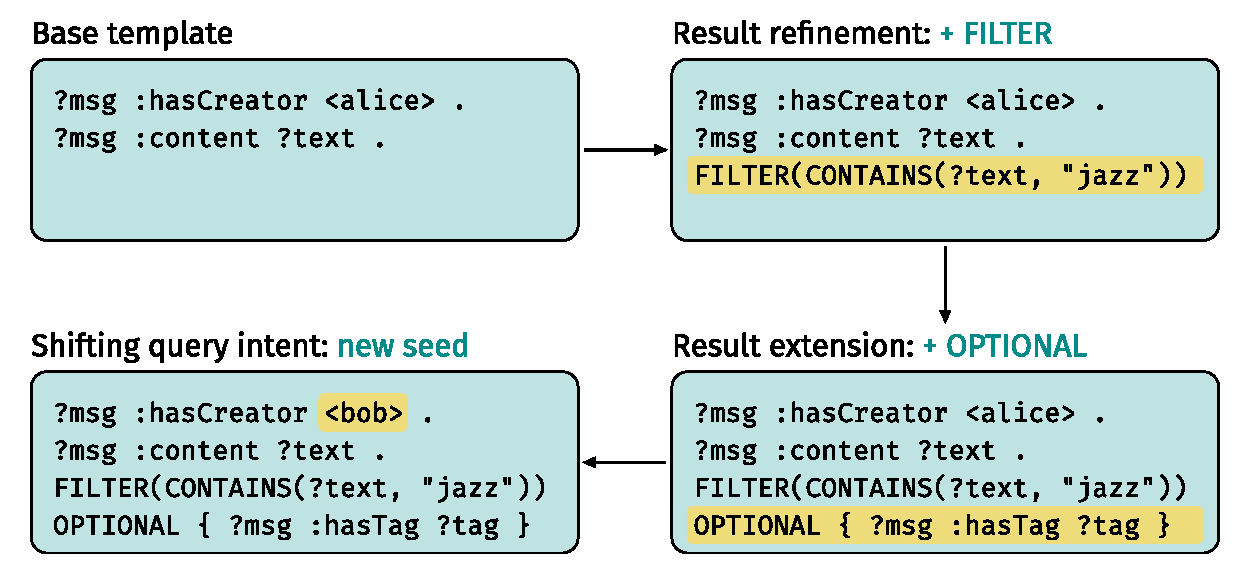
\includegraphics[width=.85\linewidth]{images/query-refinement.pdf}
\end{frame}
